\section{Introduction}
\label{sec:introduction}

% state the learning objective 
The objective of this laboratory assignment is to build an amplifying circuit based on an OP-AMP component.

As we can see in the figure \ref{fig:rc}, the circuit (similar to the one studied in the presential lab) is composed by a High Pass Filter Stage (C1 and R1), Amplification Stage (R3, R4 and a $\mu$741 OP-AMP as a non-inverting amplifier) and a Low Pass Filter Stage (R2 and C2).

\begin{figure}[h] \centering
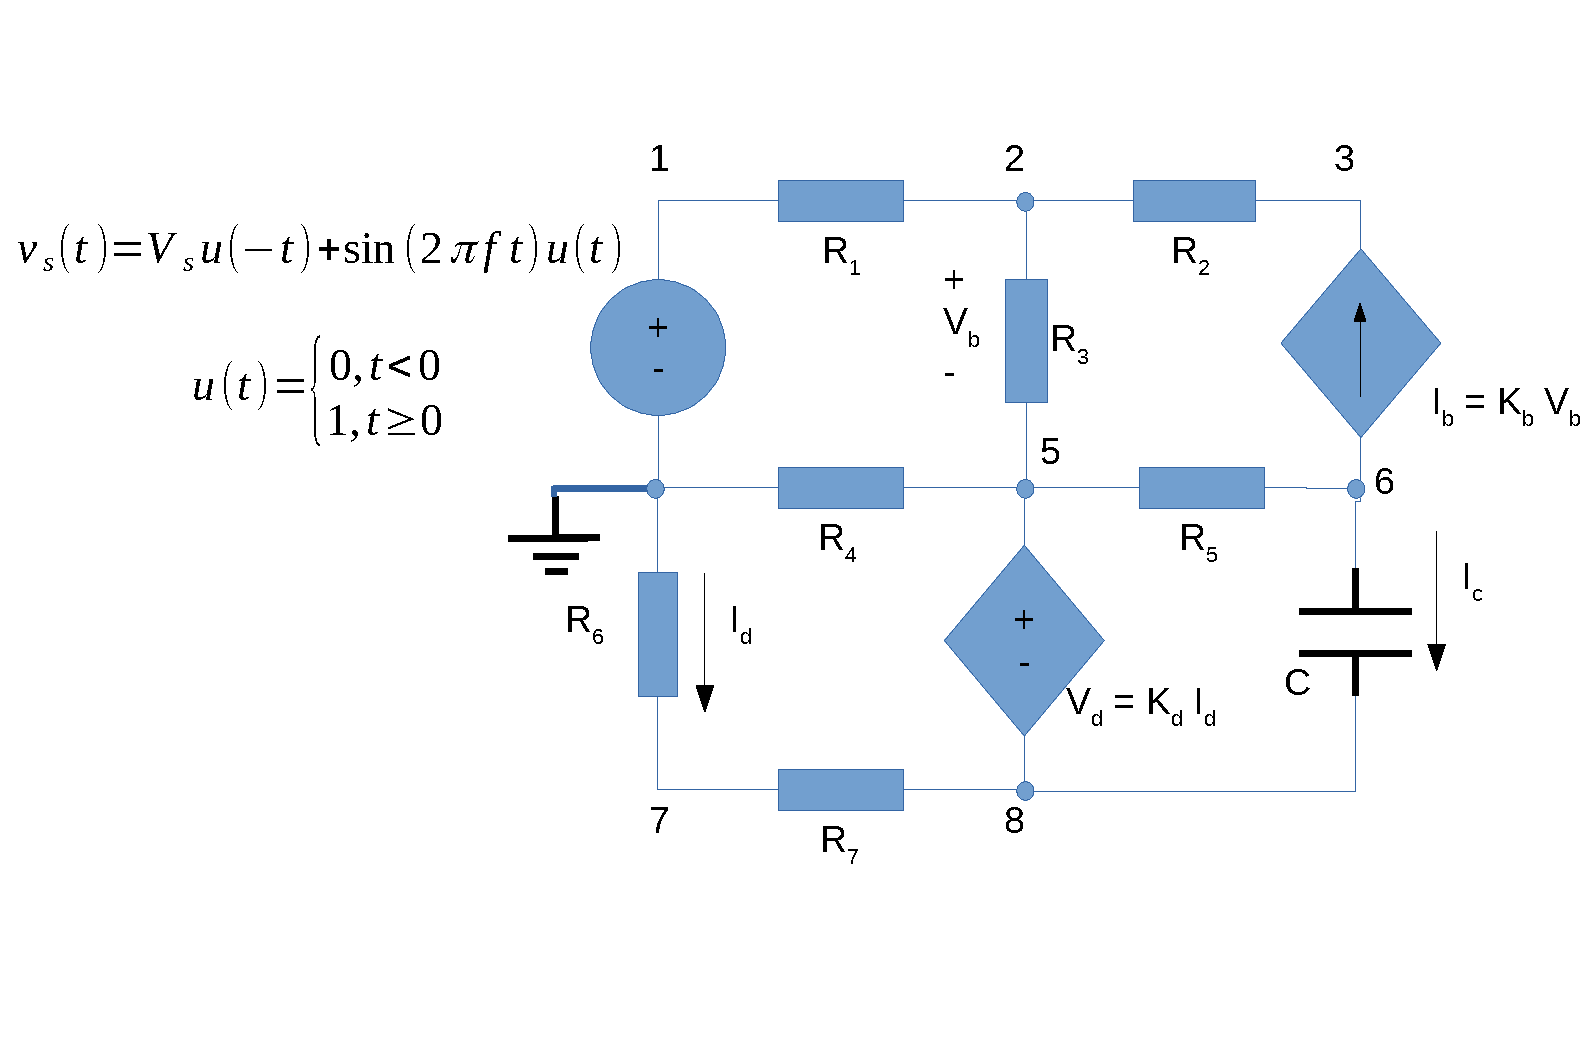
\includegraphics[width=0.99\linewidth]{rc.pdf}
\vspace{-5mm}
\caption{The Bandpass Filter}\label{fig:rc}
\end{figure}

The final values of the components used are the following:

\begin{table}[!htb]
\centering
  \begin{tabular}{|c|c|}
    \hline    
    \input{../mat/components.tex}
 \end{tabular}
 \caption{Components used in this lab assignment}\label{tab:components}
\end{table}


In Section \ref{sec:analysis}, a theoretical analysis of the circuit is presented. In Section\ref{sec:simulation}, the circuit is analysed by simulation, and the results are compared to the theoretical results obtained in Section\ref{sec:analysis}. The conclusions of this study are outlined in Section~\ref{sec:conclusion}.






